%------------------------------------------------------------------------------
% Tema 13. Osteoporosi
%------------------------------------------------------------------------------
\section{Osteoporosi}
\label{sec:osteoporosi}

La osteoporosi �s una malaltia multifactorial (m�ltiples gens i
variables ambientals). Sembla ser que la massa �ssia �s un car�cter
amb una heretabilitat important:
\begin{itemize}
\item 50-70\% en estudis intergeneracionals.
\item 80-90\% en estudis de bessons.
\item 46-62\% despr�s d'ajustar la densitat �ssia per edat, pes i
  h�bits de vida.
\end{itemize}

Hi ha dos tipus de gens que expliquen la base gen�tica de les
malalties:

\begin{enumerate}[\bf 1)]
\item \textbf{Gen d'efecte principal:} T� un efecte gran, amb
  mutacions poc freq�ents que expliquen una petita part de la
  variabilitat poblacional. Her�ncia mendeliana simple.

\item \textbf{Gens de susceptibilitat:} Tenen un efecte
  lleu. Presenten mutacions comuns, polimorfismes i expliquen una gran
  part de la variabilitat poblacional. L'her�ncia �s complexa, hi ha
  implicats molts gens, factors ambientals i interaccions gen-gen i
  gen-ambient.
\end{enumerate}

Un factor ambiental (nicotina) t� efectes sobre un TF.

\subsection{Factors per la susceptibilitat a la osteoporosi}
\label{sec:factors-per-la}

Segons l'OMS, l'osteoporosi es pot definir com un valor de DMO per
sota de 2,5 desviacions est�ndard per sota de la mitjana del pic de
massa �ssia (1 SD per osteop�nia).

\begin{figure}[H]
\centering
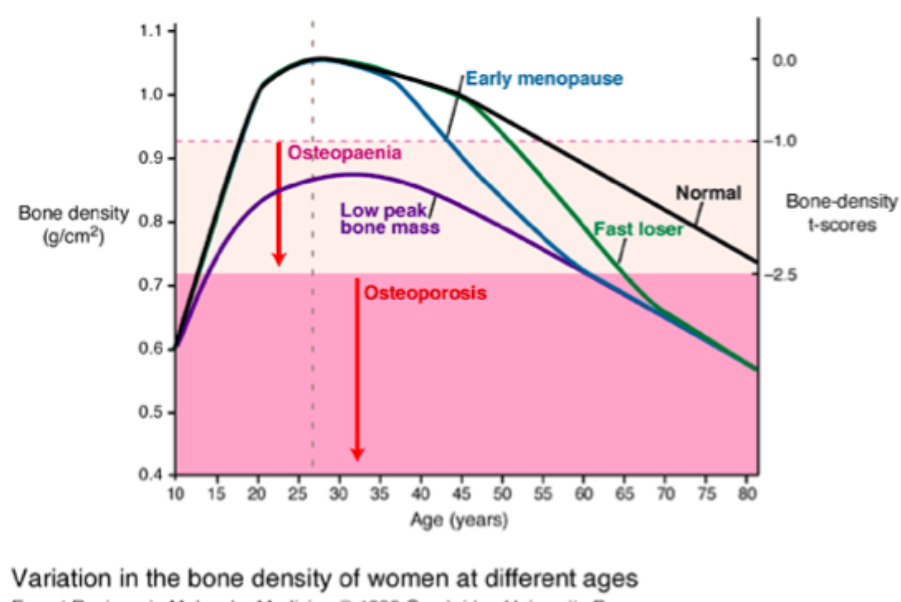
\includegraphics[width=0.8\textwidth]{fig50}
\label{fig50}
\end{figure}

Per malalties monog�niques, es fa an�lisi de lligament o WES. Per les
malalties complexes, es fa an�lisi d'associaci�, primer amb gens
candidats i despr�s per GWAS.

LRP5 es va identificar com a gen causant d'una forma d'alta densitat
�ssia monog�nica. 

Es poden fer estudis amb parelles de germans (lligament no
param�tric). Es mira si la concordan�a entre germans afectes �s m�s
gran del que s'esperaria en la poblaci� general.

\subsection{Implicaci� de polimorfismes del promotor del gen COLIA1 en
  la osteoporosi}
\label{sec:impl-de-polim}

Es van 2 nous SNPs al promotor del gen del col�gen de tipus I cadena
$\alpha$: -1997 G/T (PCOL2) i -1663indelT (PCOL1). Quan es troba un
SNP s'ha de mirar l'efecte fenot�pic per descartar que l'SNP trobat estigui en
desequilibri de lligament amb el real. PCOL2 i la interacci� dels 2
SNPs tenia un efecte significatiu sobre la densitat mineral �ssia
\citep{Garcia-Giralt2002}.

M�s tard es van fer estudis funcionals clonant els promotors contenint
els SNPs amb un reporter de luciferesa. Hi ha difer�ncies
significatives entre els clons portadors dels diferents
haplotips. Principalment es deuen al polimorfisme -1997 G /
T. L'al�lel G confereix una expressi� m�s alta del gen reporter. Sense
la regi� inhibidora es mantenen les difer�ncies entre els clons.

\subsection{An�lisis de tot el genoma}
\label{sec:analisis-de-tot}

Actualment hi ha diversos estudis a gran escala per estudiar les bases
gen�tiques de l'osteoporosi. Els gens cl�ssics que s'han estudiat s�n
VDR, ESR1, COL1A1, TGFB1, LRP5/6.

Sembla ser que hi ha un efecte protector del genotip XX pel gen ESR1
pel que fa a les fractures en general i les fractures vertebrals
\citep{Ioannidis2004}.

\nocite{Ioannidis2004}

En una segona etapa es van analitzar els gen sLRP5 i OPG. Es van
analitzar un nombre elevat d'SNP per cobrir tot el gen en blocs
haplot�pics usant un genotipat \textit{high-throughput} de la
plataforma SNPlex en una cohort de 950 pacients. Els blocs d'haplotip
queden compresos entre hotspots de recombinaci�. Aquests blocs
s'hereden conjuntament.

OPG participa en vies de senyalitzaci� osteoclasts-osteoblasts.

